\begin{frame}{Extension of PINNs for State-Space Modeling}

The PINN method is only suitable for autonomous PDEs in a bounded space-time domain.
    
Arnold and King (2021) propose a state-space model based on PINNs. This approach enables dynamic system control and state estimation and is suitable for applying the Extended Kalman Filter (EKF), using automatic differentiation to address system nonlinearities.
    
{\tiny Arnold, Florian, and Rudibert King. "State-Space Modeling for Control Based on Physics-Informed Neural Networks." \textit{Engineering Applications of Artificial Intelligence} 101 (2021): 104195. Elsevier.}
\end{frame}
    
\begin{frame}{State-Space Modeling}
    
The general state-space model is given by:
    
\begin{align}
x_{k+1} &= f(x_k, v_k) \quad (\text{State Equation})\\
y_k &= z(x_k, v_k) \quad (\text{Measurement Equation})
\end{align}
    
A classic example is the linear state-space model:
    
\begin{align*}
x_{k+1} &= A x_k + B v_k\\
y_k &= C x_k + D v_k
\end{align*}
    
where \(x_k\) is the state, \(v_k\) is the control input, and \(y_k\) is the measurement at time \(k\).
    
How can we define the state of the system in terms of a PDE solution?
\end{frame}
    
\begin{frame}{State-Space Modeling}
\framesubtitle{State Definition}
\begin{itemize}
    \item The PDE solution \(u(p, t) \approx \hat{u}(p, t)\) describes the course of a physical quantity over time and space (represented by color in the figure).
    \begin{itemize}
        \item The physical quantity has a different evolution over time depending on the position \(p\) in the space domain.
    \end{itemize}
\end{itemize}
\vspace{1cm}
\tiny{Dave, Akshay J., and Richard B. Vilim. 2024. "Physics-Informed State-Space Neural Networks for Transport Phenomena." \textit{Engineering Applications of Artificial Intelligence} 133: 108245. Elsevier.}
\end{frame}
    
\begin{frame}{State-Space Modeling}
\framesubtitle{State Definition}
\begin{figure}[H]
    \centering
    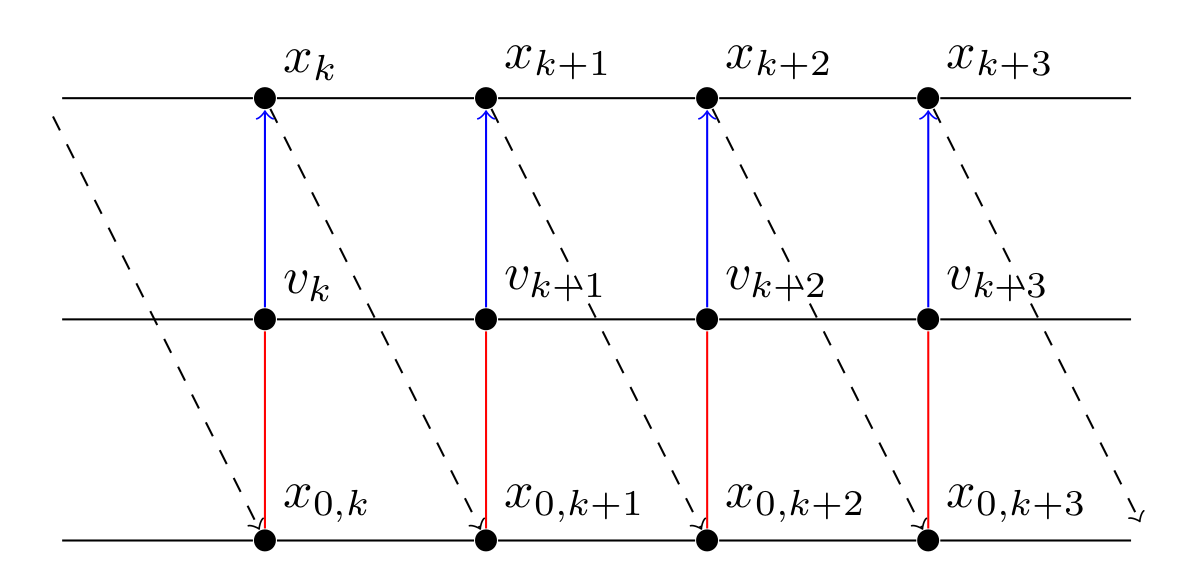
\includegraphics[width=0.8\textwidth]{img/psm.png}
    \caption{A visualization of the nomenclature and their relationships. The red lines indicate variables needed at each step \(k\), i.e., the initial condition and input, \(x_{0,k}\), and \(v_k\). The blue arrows indicate the prediction of the next state, \(x_k\), by the numerical solver or PSM. The dashed arrows indicate the aliasing of \(x_k\) as \(x_{0,k+1}\).}
\end{figure}
\end{frame}
    
\begin{frame}{State-Space Modeling}
\framesubtitle{Training Procedure}
\begin{figure}[H]
    \centering
    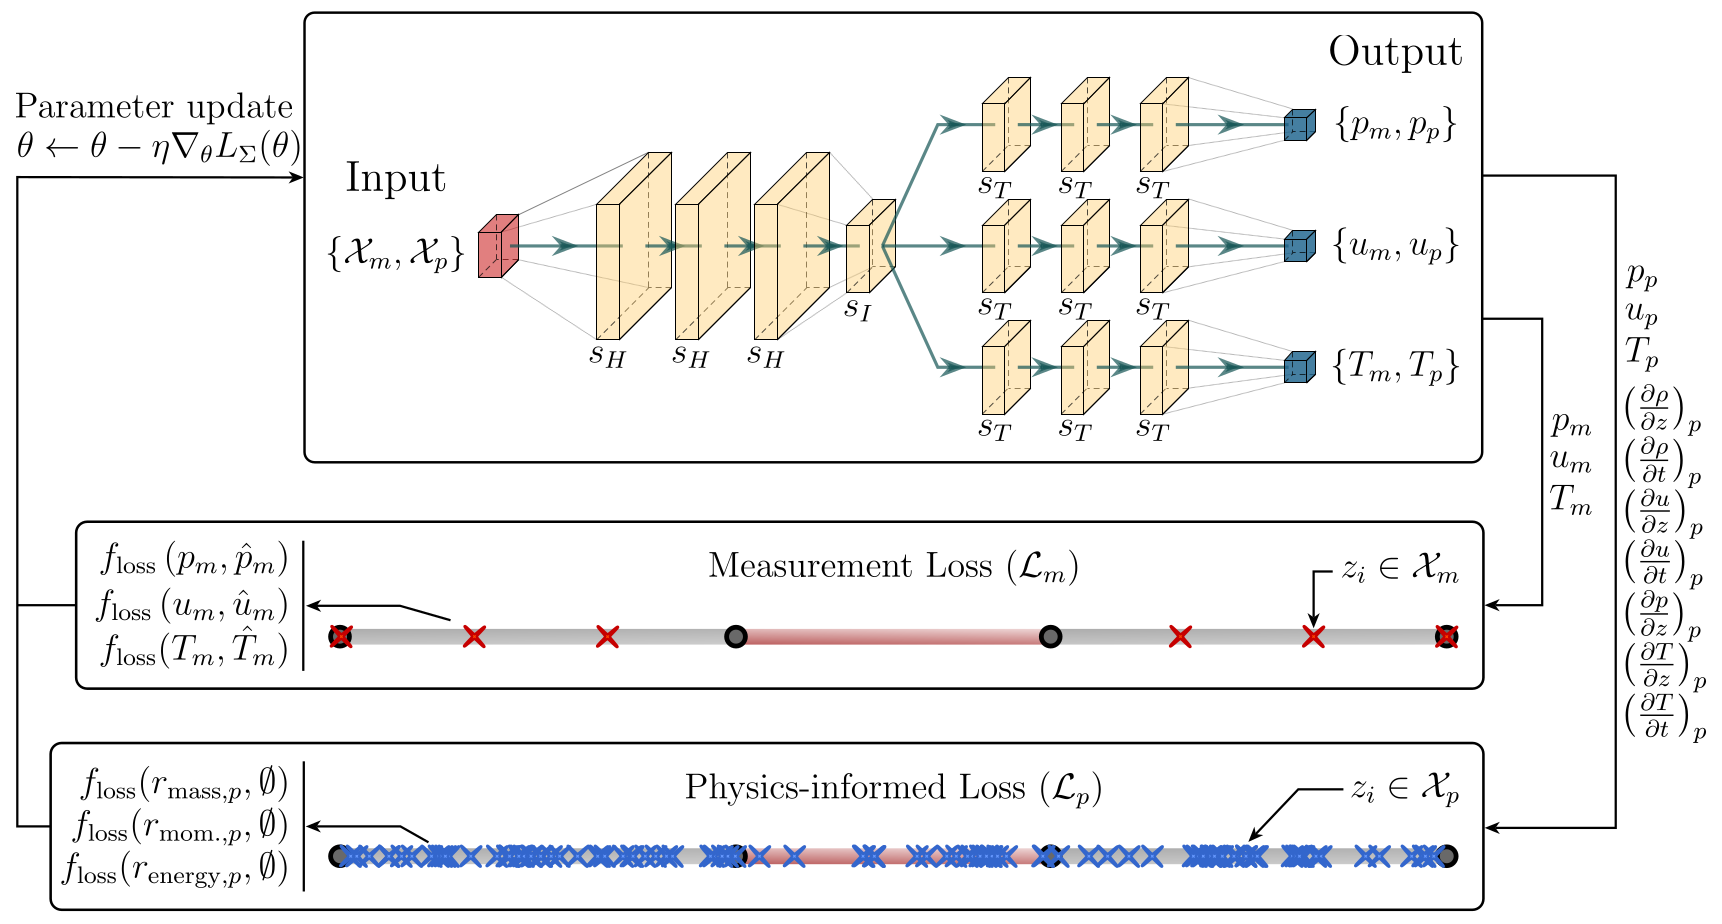
\includegraphics[width=1\textwidth]{img/psm-train.png}
\end{figure}
\end{frame}
    
\begin{frame}{Comments on the PSM approach}
\begin{itemize}
    \item In macroeconomics and finance, we observe only one realization of the measurement \(y_k\) at each time step \(k\).
    \begin{itemize}
        \item Only one realization of the state \(x_k\) may be available.
        \item The proposed estimation procedure can't be directly applied.
    \end{itemize}
    \item In the literature, these issues are addressed by using the Extended Kalman Filter (EKF) to estimate the state \(x_k\).
    \begin{itemize}
        \item The EKF is a recursive Bayesian filter that estimates the state of a dynamic system from a series of noisy measurements.
        \item Common procedure: Linearize the state-space model around the steady state.
    \end{itemize}
    \item The automatic differentiation capabilities of PINNs can help to estimate the optimal Kalman gain by circumventing the need for linearization.
\end{itemize}
\end{frame}
    